\documentclass[titlepage, letterpaper, fleqn]{article}
\usepackage[utf8]{inputenc}
\usepackage{fancyhdr} % fancy headers, of course!
\usepackage{amsmath} % what do you think?
\usepackage{amsthm} % theorems!
\usepackage{extramarks} % more cute things
\usepackage{enumitem} % i'm not sure...
\usepackage{multicol} % multicolumn...?
\usepackage{amssymb} % more symbols
\usepackage{MnSymbol} % moar symbols?
\usepackage{booktabs} % cool looking tables
\usepackage{tikz} %venn and shizzle
\usepackage{mathrsfs} %math script for calligraphic scripting, I GUESS
\usepackage{listings}
\usepackage{hyperref}
\usepackage{tcolorbox}
\usepackage{algpseudocode}
\usepackage{csquotes}

\topmargin=-0.45in
\evensidemargin=0in
\oddsidemargin=0in
\textwidth=6.5in
\textheight=9.0in
\headsep=0.25in


%
% You should change this things~
%

\newcommand{\mahteacher}{José Carlos Ortiz Bayliss}
\newcommand{\mahclass}{Computational Intelligence}
\newcommand{\mahtitle}{\textsc{Programming Assignment 03}}
\newcommand{\mahdate}{\today}

\newcommand{\spacepls}{\vspace{5mm}}
% \newcommand{\qedpls}{\blacksquare}

\renewcommand\qedsymbol{\(\blacksquare\)}
\renewcommand{\ttdefault}{pcr} %so we can get both bold and tt fonts

\newcommand{\bigO}{\mathcal{O}} %you should be inside a math environment
%
% Header markings
%

\pagestyle{fancy}
\lhead{01170065 - Xavier Sánchez}
\chead{}
\rhead{}
\lfoot{}
\rfoot{}


\renewcommand\headrulewidth{0.4pt}
\renewcommand\footrulewidth{0.4pt}

\setlength\parindent{0pt}
% \setlength\parskip{1.5pt}
\setlength\parskip{1.5ex}


%
% Create Problem Sections (stolen directly from jdavis/latex-homework-template @ github!)
%

\newcommand{\enterProblemHeader}[1]{
\nobreak\extramarks{}{Problem \arabic{#1} continued on next page\ldots}\nobreak{}
\nobreak\extramarks{Problem \arabic{#1} (continued)}{Problem \arabic{#1} continued on next page\ldots}\nobreak{}
}

\newcommand{\exitProblemHeader}[1]{
\nobreak\extramarks{Problem \arabic{#1} (continued)}{Problem \arabic{#1} continued on next page\ldots}\nobreak{}
\stepcounter{#1}
\nobreak\extramarks{Problem \arabic{#1}}{}\nobreak{}
}

\setcounter{secnumdepth}{0}
\newcounter{partCounter}
\newcounter{homeworkProblemCounter}
\setcounter{homeworkProblemCounter}{1}
\nobreak\extramarks{Exercise \arabic{homeworkProblemCounter}}{}\nobreak{}

%Solution Environment
% \newenvironment{solution}
% {\renewcommand\qedsymbol{$\square$}\begin{proof}[Solution]}
% {\end{proof}}

% Alias for the Solution section header
\newcommand{\solution}{\textbf{\Large Solution}}

%Alias for the new step section
\newcommand{\steppy}[1]{\textbf{\large #1}}

%
% Homework Problem Environment
%
% This environment takes an optional argument. When given, it will adjust the
% problem counter. This is useful for when the problems given for your
% assignment aren't sequential. See the last 3 problems of this template for an
% example.
%
\newenvironment{homeworkProblem}[1][-1]{
\ifnum#1>0
\setcounter{homeworkProblemCounter}{#1}
\fi
\section{Problem \arabic{homeworkProblemCounter}}
\setcounter{partCounter}{1}
\enterProblemHeader{homeworkProblemCounter}
}{
\exitProblemHeader{homeworkProblemCounter}
}

%
% Coloring of code listings
%

%New colors defined below
\definecolor{codegreen}{rgb}{0,0.6,0}
\definecolor{codegray}{rgb}{0.5,0.5,0.5}
\definecolor{codepurple}{rgb}{0.58,0,0.82}
\definecolor{backcolour}{rgb}{0.98,0.98,0.98}

%Code listing style named "mystyle"
\lstdefinestyle{mystyle}{
  backgroundcolor=\color{backcolour},
  commentstyle=\color{codegreen},
  keywordstyle=\bfseries\color{blue},
  numberstyle=\tiny\color{codegray},
  stringstyle=\color{codepurple},
  basicstyle=\footnotesize\ttfamily,
  breakatwhitespace=false,         
  breaklines=true,                 
  captionpos=b,                    
  keepspaces=true,                 
  numbers=left,                    
  numbersep=5pt,                  
  showspaces=false,                
  showstringspaces=false,
  showtabs=false,                  
  tabsize=2
}

%"mystyle" code listing set
\lstset{style=mystyle}

%
% My actual info
%

\title{
\vspace{1in}
\textbf{Tecnológico de Monterrey} \\
\vspace{0.5in}
\textmd{\mahclass} \\
\vspace{0.5in}
\large{\textit{\mahteacher}} \\
\vspace{0.5in}
\textsc{\mahtitle}\\
\author{01170065  - MIT \\
Xavier Fernando Cuauhtémoc Sánchez Díaz \\
\texttt{xavier.sanchezdz@gmail.com}}
\date{\mahdate}
}

\begin{document}

\begin{titlepage}
\maketitle
\end{titlepage}

%
% Actual document starts here~
%

\begin{homeworkProblem}

{\large \textbf{Multi-layer perceptron}}

\begin{itemize}
  \item A multi-layer perceptron was implemented using the code provided.
  The perceptron correctly classifies \texttt{dataset-PA02.csv}.
  \item The code was implemented in Octave, using the codes provided.
  \item A \texttt{readme.txt} file is included with the details needed for execution, along with the Texinfo per-module documentation, i.e. you can use \texttt{help PA03} in the Octave prompt for instructions.
\end{itemize}

{\large \textbf{Run details}}

The code \texttt{PA03(data, 1, 'c', 2, 0.1, 1000, 20)} correctly classified the dataset at run 18 with the following parameters:

$$W1 =
\begin{bmatrix}
1.68740 & -0.97069 \\
2.26922 & -1.68538
\end{bmatrix}, \quad
b1 =
\begin{bmatrix}
-1.0578 \\
1.3578
\end{bmatrix},\quad
W2 = [-1.4709, 1.2349], \quad
b2 = 0.0024276$$
\end{homeworkProblem}

\begin{homeworkProblem}
The same story goes for problem number two, but instead a 4-attribute dataset was used (\texttt{Iris.csv}).

{\large \textbf{Run details}}

The code \texttt{PA03(data\_iris, 2, 'c', 0.1, 1000, 20)} correctly classified the dataset at run 7 with the following parameters:

$$W1 =
\begin{bmatrix}
  0.597255 & 0.911574 & 0.699710 & 0.057203 \\
  0.626836 & 0.237436 & 0.765186 & 0.088687
\end{bmatrix}, \quad
b1 =
\begin{bmatrix}
  0.038780 \\
  0.041295
\end{bmatrix}, \quad
W2 = [-0.23743, 0.42891], \quad
b2 =  0.30965$$
\end{homeworkProblem}

\begin{homeworkProblem}

The neural network was trained using the regression mode in order to approximate the function values available in \texttt{dataset-function.csv}.

The following parameters were used:

\begin{lstlisting}
PA03(datafn, 3, 'r', 3, 0.01, 5000, 1); hold on; plot(datafn(:,2)); grid;
\end{lstlisting}

$$W1 =
\begin{bmatrix}
  -2.1291 \\
   5.3270 \\
   7.6768
\end{bmatrix}, \quad
b1 =
\begin{bmatrix}
   -4.0754 \\
  -13.6089 \\
   21.0353
\end{bmatrix}, \quad
W2 =[-23.278, 18.499, 14.685], \quad
b2 = -15.861$$

As seen on  the listing presented below,
the number of iterations was increased in order for 3 neurons to acquire a good approximation.
Figures~\ref{fig:2n}~\ref{fig:3n} show these behavior.

\begin{figure}[htbp]
  \centering
  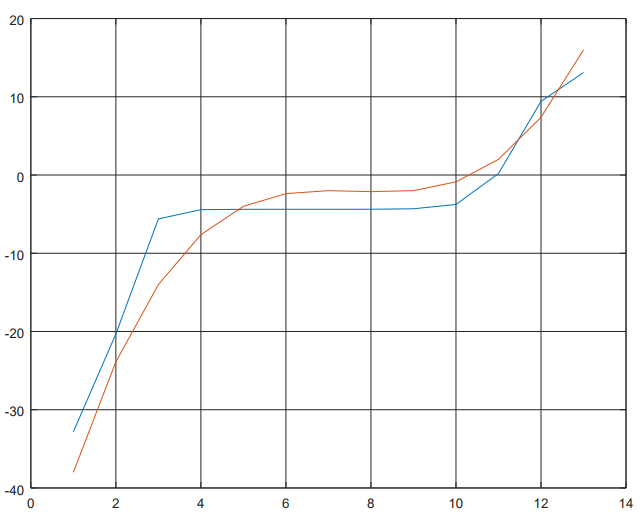
\includegraphics[width=0.7\textwidth]{Ex3-2n.png}
  \caption{2-neuron function approximation}
  \label{fig:2n}
\end{figure}

\begin{figure}[htbp]
  \centering
  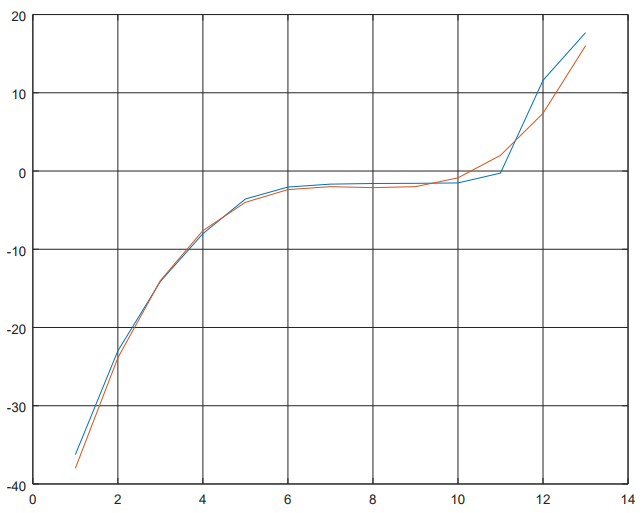
\includegraphics[width=0.7\textwidth]{Ex3-3n.png}
  \caption{3-neuron function approximation}
  \label{fig:3n}
\end{figure}

Using a higher number of neurons can provide softer edges for the function approximation model.
The ``best'' results would be using 13 neurons, as there were 13 rows in the dataset: a neuron per datum.
This is an extreme assumption, but it shows the basic idea behind overfitting.
\end{homeworkProblem}

\begin{homeworkProblem}
If the dataset is divided by 10, the model finds it more difficult to approximate the function.

The values are too close from each other, and experimental results show that the model needed twice the training iterations that it used for the previous dataset.

\begin{lstlisting}
PA03(datafn2, 3, 'r', 3, 0.01, 20000, 1); hold on; plot(datafn2(:,2)); grid  
\end{lstlisting}

Since the values are so close, the model need additional time to `learn' the differences between values.
This means that increasing the number of neurons is useful when dealing with `difficult' problems, with many different features to remember.
However, this increases the time needed for appropriate learning.
It is also important to take into account that a neuron is adding bias to the model,
so more biases means a more specific model---one should be careful with overfitting.
\end{homeworkProblem}



\end{document}